\chapter{Introduction}\label{cap:introduction}

\todo[inline]{TODO: Expand and refine the Introduction chapter.}

Forests are a crucial part of the global ecosystem, both environmentally and economically.
They cover a third of the land area, contain over 80\% of terrestrial biodiversity, and somewhere around one-third of humanity depends on forests and forest products for their livelihoods \cite{aertsForestRestorationBiodiversity2011, StateWorldsForests2020}.
Forests are an essential renewable natural resource and a huge, dynamic part of the global carbon cycle.
Responsible management of forests allows using the resources efficiently and sustainably, preserving the biodiversity, and regulating atmospheric $CO_2$, which is becoming especially important as the anthropogenic climate change is ongoing and accelerating \cite{faheyForestCarbonStorage2010, forsterIndicatorsGlobalClimate2024}.
This drives the need for accurate, detailed, up-to-date information about various forest attributes such as distributions of tree species, average heights and ages of trees, estimates of trunk diameter, timber volume, and above ground biomass, and others.

The traditional manual forest inventories are extremely labor-intensive and time-consuming, which makes them infeasible to cover extensive areas with sufficient detail, speed, and frequency \cite{burleyEncyclopediaForestSciences2004}.
Various remote sensing techniques are widely used to extend and extrapolate manual inventories.
All sorts of data, from satellite and aerial imagery to very detailed terrestrial LiDAR surveys, are used in all sorts of applications that require mapping forest attributes.


There are even many free data sources such as Sentinels (some studies of using S1 and S2, maybe even GEDI).
Higher resolution data is however only available for money, and it isn't cheap.

The most common way to use LiDAR surveys for mapping forest attributes in industry is the area-based approach described in detail in Section~\ref{sec-area-based-approach}.

However, modern sensors and processing techniques allow not aggregating at all and instead working on the level of individual trees.
This requires robust algorithms that allow detecting individual trees in dense multimodal data.
This is relatively easy in urban environments, manually planted and managed forest stands, or forests that are either sparse or predominantly coniferous, where the structure of the canopy is easy to interpret.
Forest that are mixed and dense are much harder to work with and are a very active area of research for developing methods of detection of individual trees.

The framework described in this thesis focuses on fusion of two remote sensing data sources: UAV LiDAR point clouds and UAV RGB orthophotos.
The choice is explained mostly by practicality.

LiDAR is an active sensor, which means it does not depend on external conditions such as lightning.

UAV measurements offer a good balance between the affordability, required effort, and quality of the data.

The main research question ...
The main hypothesis is ...
Significantly reduce the required effort, especially in the form of the amount of field inventory data required.
Ideally, a method that doesn't require any field data at all, only for validation and quality assessment.
Match or exceed the accuracy of the area-based approach.

The proposed framework described in this thesis consist of a neural-network based tree segmentation in UAV LiDAR point clouds enhanced with RGB orthophoto-based features and processing the segments with a collection of specialized classic machine learning models that predict the parameters of interest for each detected tree.
The tree segmentation model is trained on synthetic forest patches constructed from a dataset of point clouds of individual trees extracted manually from a large UAV LiDAR survey, heavily relying on augmentations to make the synthetic forest closer to real forest.
The parameter prediction classification and regression models are trained on the same dataset of individual trees using a collection of widely used manual point cloud features.
Figure~\ref{fig-framework-apply} is a schematic representation of the framework, showing the required inputs in red, processing steps in yellow, and artifacts in cyan.

\begin{figure}
\centering{
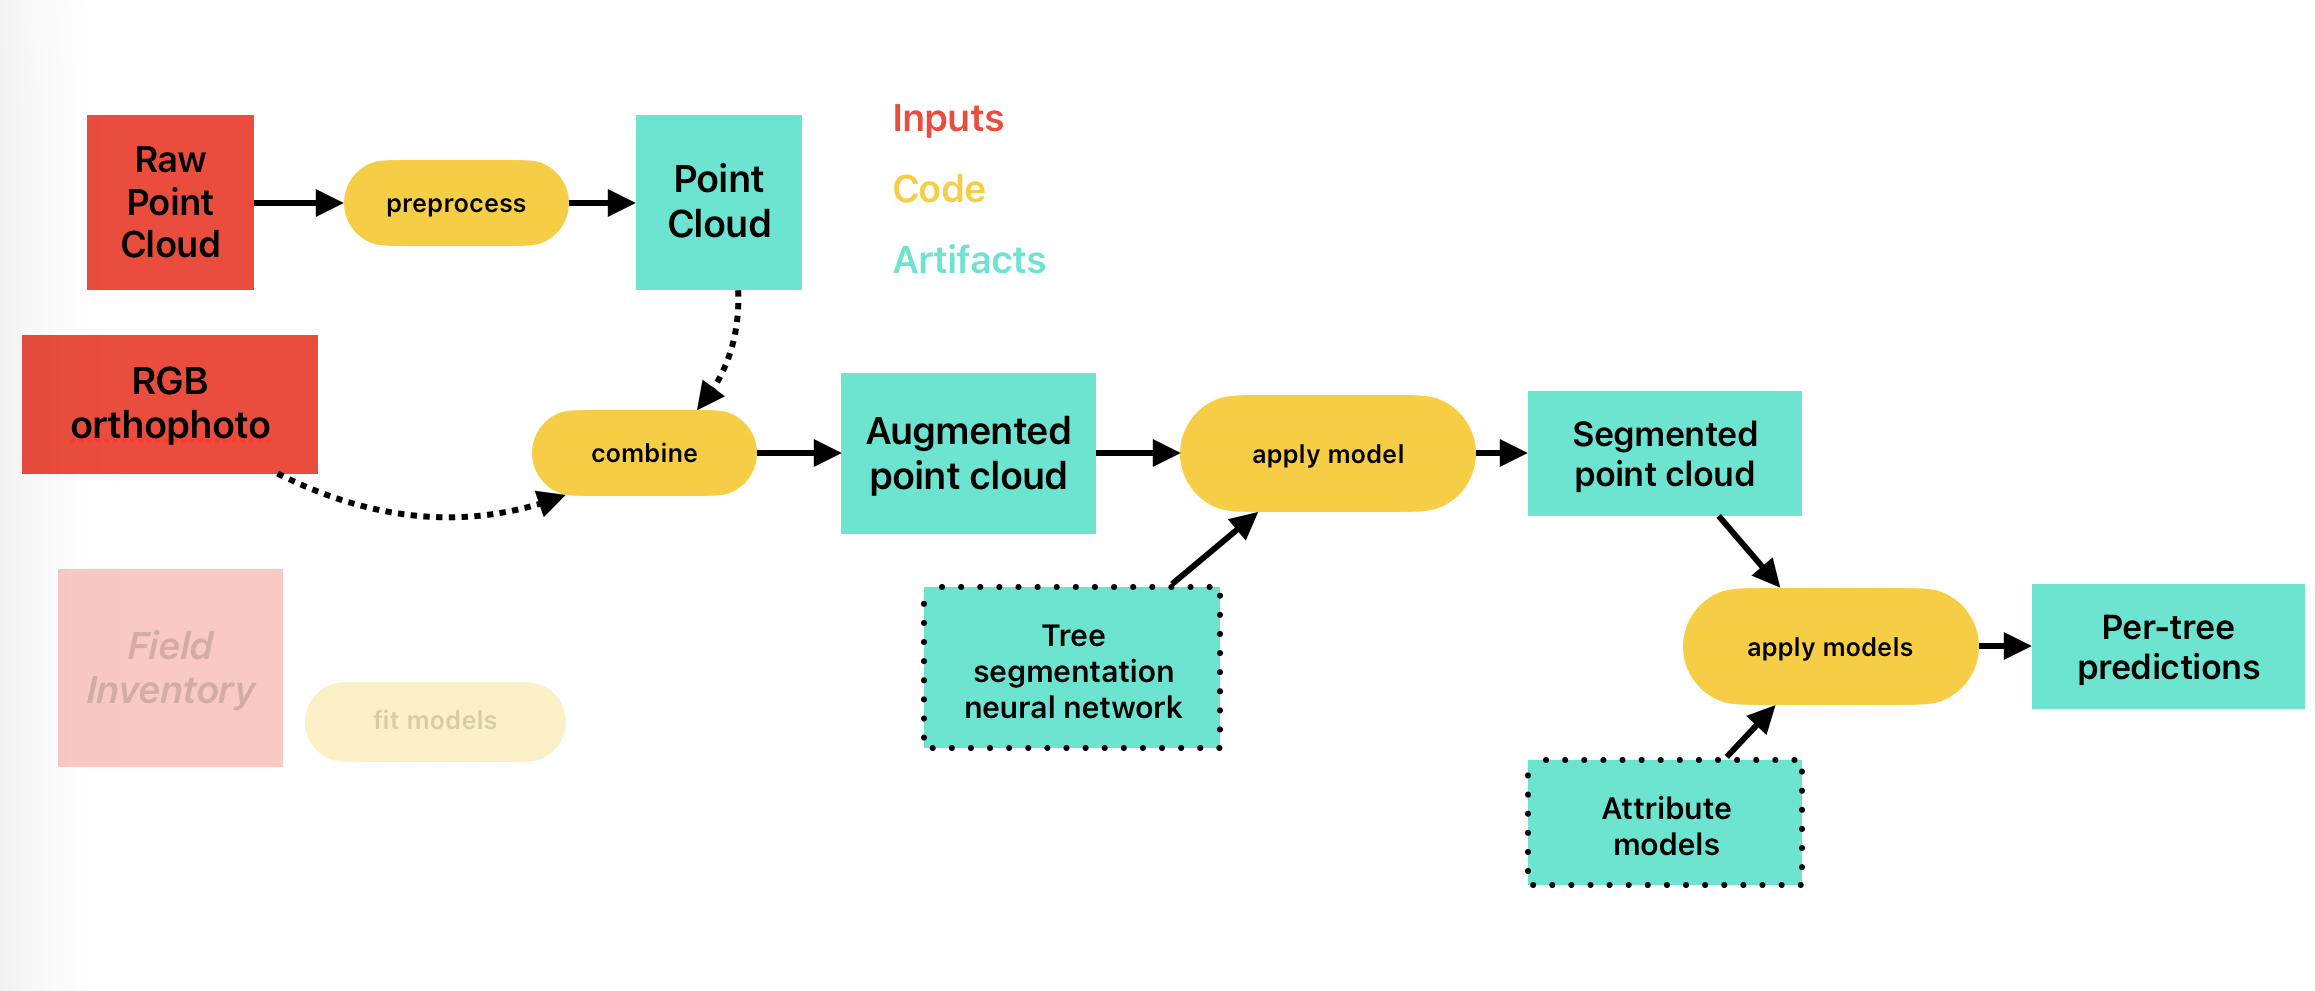
\includegraphics[width=\textwidth]{../images/framework_application_schematic.jpg}
}
\caption{\label{fig-framework-apply}The schematic representation of the
framework in the application stage.}
\end{figure}

Figure~\ref{fig-framework-prepare} is a schematic of the preparation
step for the framework.

\begin{figure}
\centering{
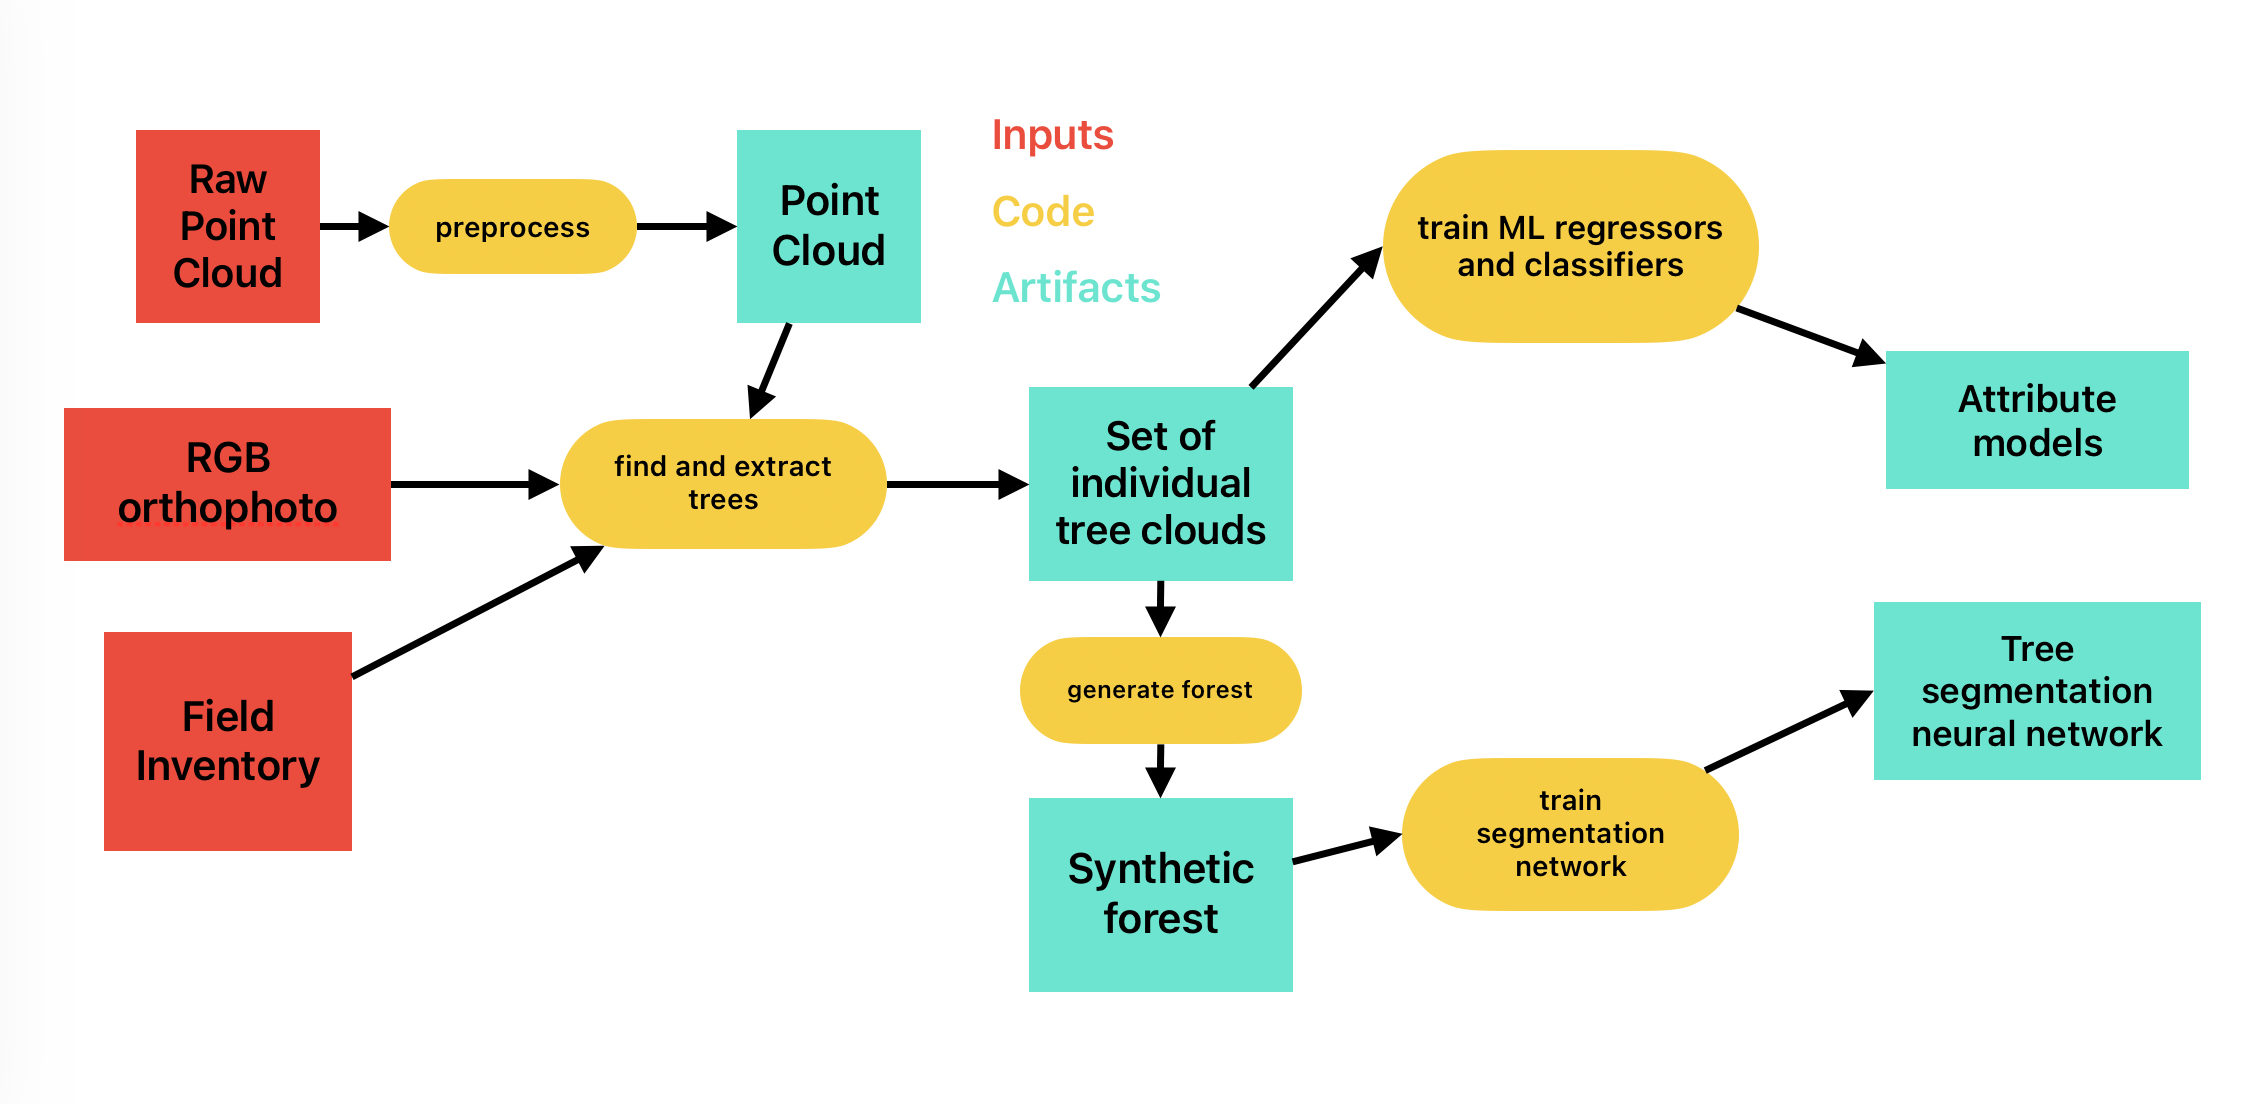
\includegraphics[width=\textwidth]{../images/framework_preparation_schematic.jpg}
}
\caption{\label{fig-framework-prepare}The schematic representation of
the framework in the preparation stage.}
\end{figure}

\section{Thesis Structure}

\begin{description}
    \item[\Autoref{cap:introduction} - Introduction]
The Introduction chapter aims to give a general introduction to the research project and put it into wide scientific and societal context.
It defines the main research question and the hypothesis, and gives a high-level overview of the proposed framework.
It also provides the links to the original datasets and the code.

    \item[\Autoref{cap:literature} - Literature Review]
The Literature Review chapter aims to give an overview of the scientific literature on topics most relevant to the project.
Its main goals are to provide the reader with context for the research described in the thesis, provide references for in-depth materials on topics that are out of scope of this work, and to highlight the research gap that the work tries to address.

	\item[\Autoref{cap:materials} - Materials and methods]
The Materials and Methods chapter describes in detail the datasets, methods and methodological choices used in the proposed framework.
It's aim is to make the work reproducible and to explain the methodological choices made.

	\item[\Autoref{cap:results} - Results]
The Results chapter describes the results of each stage of the framework preparation and the validation approach used to verify its applicability and effectiveness on realistic data.

    \item[\Autoref{cap:conclusion} - Conclusion]
The Conclusion chapter offers a brief summary of the thesis as a whole, potential perspectives for further improvement of the proposed framework, and some concluding thoughts.

\end{description}

\section{Data and code availability}

Original datasets described in the thesis are openly available on Kaggle \href{https://www.kaggle.com/datasets/sentinel3734/tree-detection-lidar-rgb}{here} and \href{https://www.kaggle.com/datasets/sentinel3734/uav-point-clouds-of-individual-trees}{here}.
All the code used for the project is available on GitHub at \href{https://github.com/iod-ine/phd}{iod-ine/phd}.
The thesis document was developed using Quarto \cite{Allaire_Quarto_2024} using the literate programming approach \cite{knuth84}, and a link to an HTML version hosted through GitHub Pages is available in the repository.
The deep learning part is implemented using PyTorch \cite{Ansel_PyTorch_2_Faster_2024}, PyTorch Geometric \cite{Fey_Fast_Graph_Representation_2019}, and PyTorch Lightning \cite{Falcon_PyTorch_Lightning_2019}, with experiment tracking using MLflow.
Classic machine learning models implementations are from scikit-learn \cite{scikit-learn}.
NumPy \cite{2020NumPy-Array}, SciPy \cite{2020SciPy-NMeth}, pandas \cite{The_pandas_development_team_pandas-dev_pandas_Pandas}, scikit-image \cite{van_der_Walt_scikit-image_image_processing_2014} libraries are used for processing the data.
ratserio \cite{gillies_2019}, geopandas, laspy, lazrs libraries are used for working with geospatial data formats.
matplotlib \cite{Hunter_Matplotlib_A_2D_2007} and seaborn \cite{waskomSeabornStatisticalData2021} libraries are used for visualization.
